
\chapter{Aufgabestellung}\label{chp:aufgabenstellung}
\paragraph{}

Ziel dieser Masterarbeit ist die Verbesserung der Testfallgenerierung und der Testabdeckung bei mehreren Produktvarianten, die Ersetzung von Parameter, die Prozessoptimierung sowie die Handhabung für den Benutzer in der TESTONA-Umgebung. Jedes Produkt kann unterschiedliche Produktvarianten beinhalten und jede Variante besteht aus unterschiedlichen Komponenten mit unterschiedlichen Parametern. In Abhängigkeit von der ausgewählten Variante sollen bei der Testfallgenerierung die dazugehörigen Komponenten berücksichtigt werden und die erzeugten Testfälle dargestellt werden. Besonders zu beachten sind dabei die definierten Abhängigkeitsregeln sowie die darauf bezogene Testabdeckung.\\

Abhängigkeitsregeln werden definiert um redundante Testfälle zu vermeiden, bzw. um Vorbedingungen für die Testfälle zu erstellen. Da Varianten verschiedene Baumelemente beinhalten, kann es dazu kommen, dass Baumelemente für Abhängigkeitsregeln nicht vorhanden sind. Dadurch könnte TESTONA bei der Testfallgenerierung die Testabdeckung verfälschen, indem die Gültigkeit eines Testfalles nicht garantiert werden kann. Um dieses Problem zu umgehen, muss bei der Erzeugung von Abhängigkeitsregeln auf mögliche Konflikte hingewiesen werden. Für den Lösungsansatz gibt es verschiedene Thesen die analysiert werden müssen, um eine optimale Prozessoptimierung zu erreichen.\\

Um die Handhabung der Varianten bezogen auf die Testfälle und die Testgenerierung benutzerfreundlicher und effizienter zu gestalten, soll die Benutzung des Variantenmanagements durch einen Testingenieur untersucht werden. Resultierend aus den erworbenen Erkenntnissen wird das Lösungsdesign für eine Erweiterung des bestehenden Variantenmanagements in TESTONA konzipiert.\\

Einer der besonderen Eigenschaften von TESTONA ist die Kopplung mit Anforderungsspezifikationen die in IBM Rational DOORS definiert worden sind. Durch das DOORS Add-On MERAN können Anforderungen die in DOORS definiert sind, mit den zugehörigen Varianten verknüpft werden. Diese Varianten können in TESTONA eingebunden werden, durch eine erfolgreiche Anmeldung bei DOORS (über die TESTONA Oberfläche) und ein gezieltes Auswählen der gewünschten Varianten. Hierbei sollen die in den Anforderungen definierten Variablen (z.B. eine Geschwindigkeit oder Anzahl der Türen eines Autos) mit gespeichert werden. Im Klassifikationsbaum soll je nach ausgewählter Variante (z.B. der Name von Klassen) mit dem entsprechenden Wert ersetzt werden. Andere Lösungsmöglichkeiten werden noch untersucht.\\

Der derzeitige Varianten-Management-Ansatz in TESTONA ist nicht in der Lage für die Testfallgenerierung zwischen verschiedene Varianten zu unterscheiden. Zwar werden durch die Perspektive „Variant Management“ verschiedene Varianten unterschieden, aber die Testfälle müssen manuell mit den jeweiligen Varianten verknüpft werden. Im Falle einer automatischen Testfallgenerierung werden auch ungültige Baumelemente betrachtet (siehe Abbild \ref{ttn.gruen} und \ref{ttn.rot}). Um dies zu vermeiden muss der Testingenieur einzelne Generierungsregeln anlegen. Dieser Vorgang soll automatisiert und von TESTONA übernommen werden. Dabei gibt es verschiedene Betrachtungsweisen und mehrere Lösungswege. Entscheidend für die Lösung werden die erworbenen Kenntnisse über die Benutzung des Variantenmanagements durch einen Testingenieurs. Bei der Lösung ist zu beachten, dass eine komplette Testfallabdeckung garantiert werden muss.\\


\begin{figure}[h]
  \begin{center}
    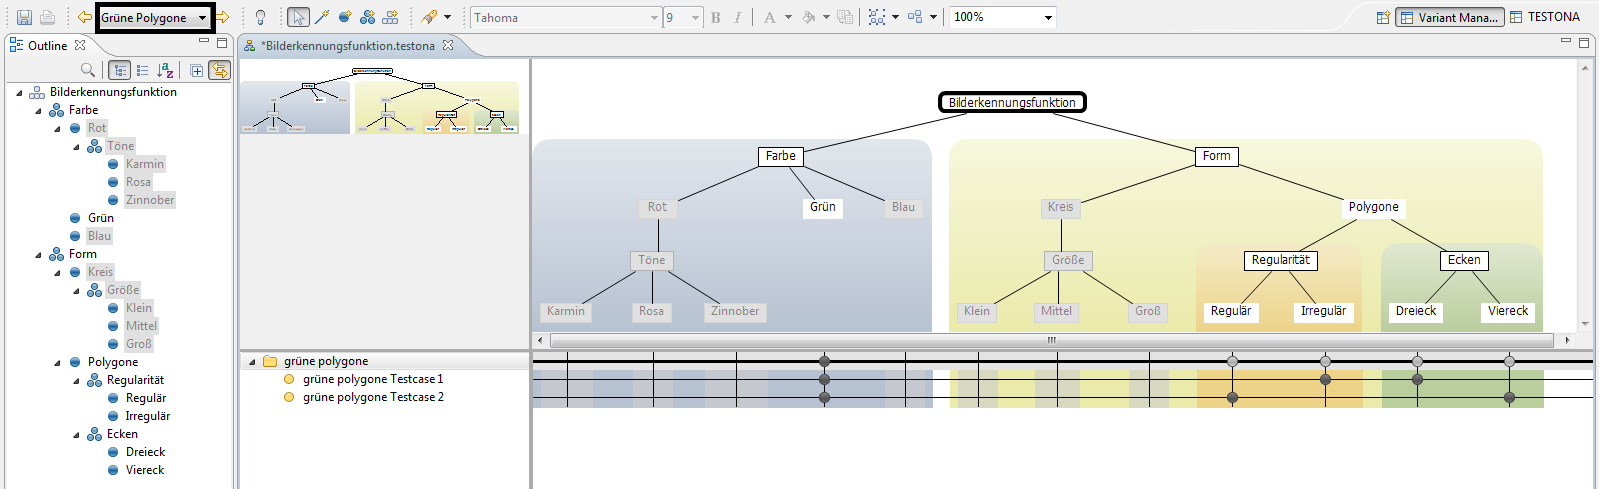
\includegraphics[scale=0.35]{gruenePolygone_DE.png}
  		  \caption{Richtige Auswahl der Klassen und Klassifikationen für die Testfallgenerierung}
     \label{ttn.gruen}
  \end{center}
\end{figure}


\begin{figure}[h]
  \begin{center}
    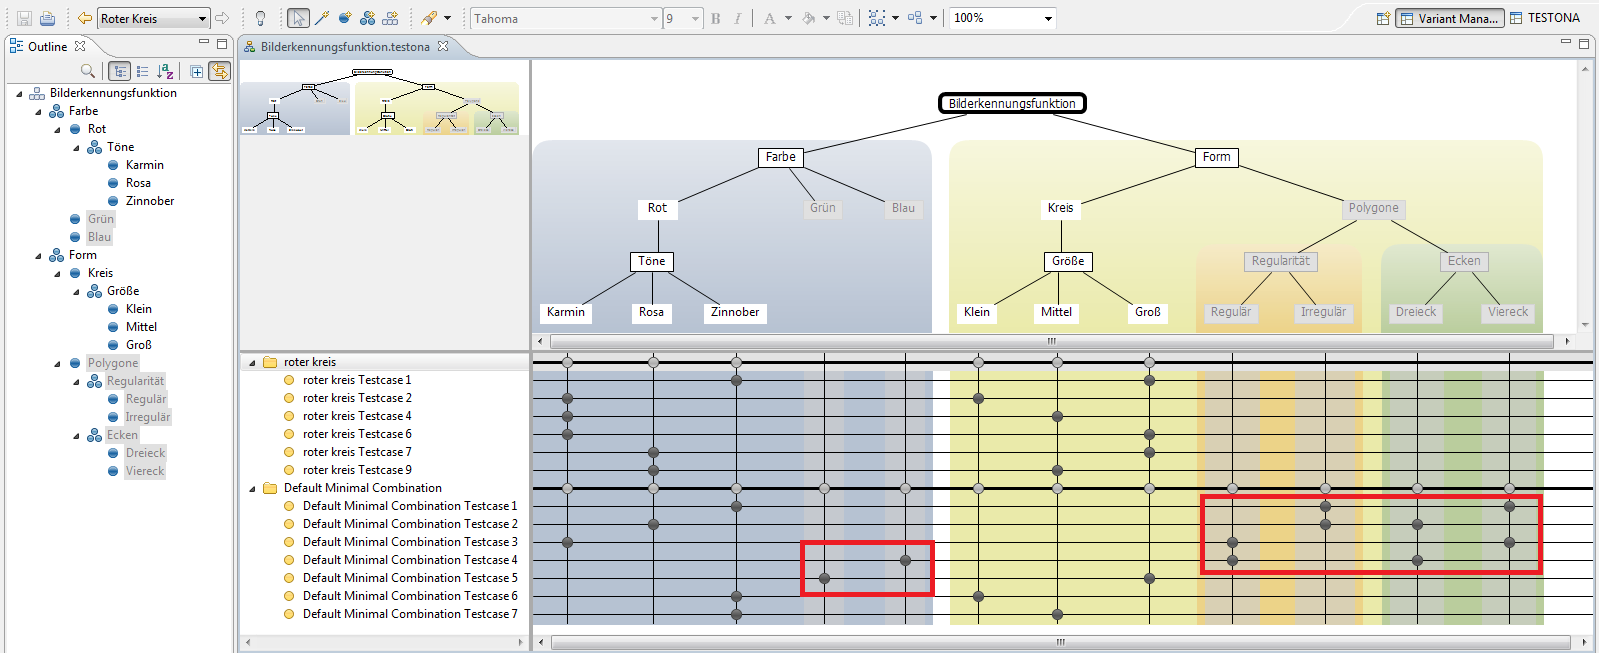
\includegraphics[scale=0.35]{roterKreis_DE.png}
  		  \caption{Ungültige Auswahl der Klassen (Grün und Blau) und Klassifikationen (Regularität und Ecken) für die Testfallgenerierung}
     \label{ttn.rot}
  \end{center}
\end{figure}


